\documentclass[10pt]{article}
\usepackage{icmlko}

\icmlmeta{IP 파운데이션 월드모델}{119}{같은 플랫폼이라 잘 맞았다}{라벨을 두 플랫폼 평균으로 보정하자 신뢰도는 올랐는데 전이가 내렸다 --- 축이 전부 같은 곳에서 나왔기 때문이고, 자기 $\rho$의 23\%가 그 정합이었다}

\begin{document}

\twocolumn[
\icmlheader

\begin{abstract}
노트 118이 ``시끄러운 것은 축이 아니라 라벨''이라 했다. 그러면 축을 더 찾는
대신 라벨을 덜 시끄럽게 만들면 된다. Kitsu \texttt{userCount} 와 AniList
라벨의 순위 상관이 \textbf{$+$0.607}이고(id 대응 2,892건 --- 노트 79 · 83의
제목 대조 $+$0.555보다 깨끗하다), 스피어만-브라운으로 두 측정의 평균은 신뢰도를
\textbf{0.756}으로 올린다. \textbf{천장이 0.779에서 0.869로 오를 터였다.}
바꿔 봤다. \textbf{전이가 내린다} --- 세계애니를 출처로 쓸 때 아홉 대상 중
여덟이 나빠지고 평균 $-$0.0068, 팝업 $-$0.0114다. 채택 0/4. 왜인지 파 보니
답이 하나였다. \textbf{축이 전부 AniList 에서 나왔다.} 태그 수 · 화수 · 연령
등급 · 외부 링크 --- 전부 같은 API 의 필드다. 축과 AniList 라벨의 상관이
$+$0.12$\sim+$0.59인데 같은 축과 Kitsu 라벨은 $+$0.02$\sim+$0.33이고
\textbf{미디어 홍보는 $+$0.460에서 $-$0.113으로 부호까지 뒤집힌다.}
자기 $\rho$로 재면 크기가 나온다 --- AniList 라벨 0.5437, 두 플랫폼 평균
0.4919, \textbf{Kitsu 라벨 0.4175}. \textbf{자기 $\rho$의 23\%가 같은 플랫폼
정합이다.} 그리고 열 도메인 중 \textbf{여덟}이 축과 라벨이 같은 플랫폼이다.
\textbf{누수와 정합은 같은 것의 두 얼굴이다} --- 노트 117에서 AniList
즐겨찾기가 AniList 라벨을 잘 맞힌 것을 누수라 불렀고, 여기서 AniList 축들이
AniList 라벨을 잘 맞히는 것을 정합이라 부른다. 정도의 차이일 뿐이다.
\textbf{그리고 팝업만 다르다} --- 축은 사람이 기획서를 읽고 매기고 라벨은
결과보고서에서 온다. \textbf{팝업의 낮아 보이는 자기 $\rho$는 팝업이 나빠서가
아니라 팝업만 정직하게 재지기 때문일 수 있다.}
\end{abstract}
]

\begin{figure*}[t]
\centering
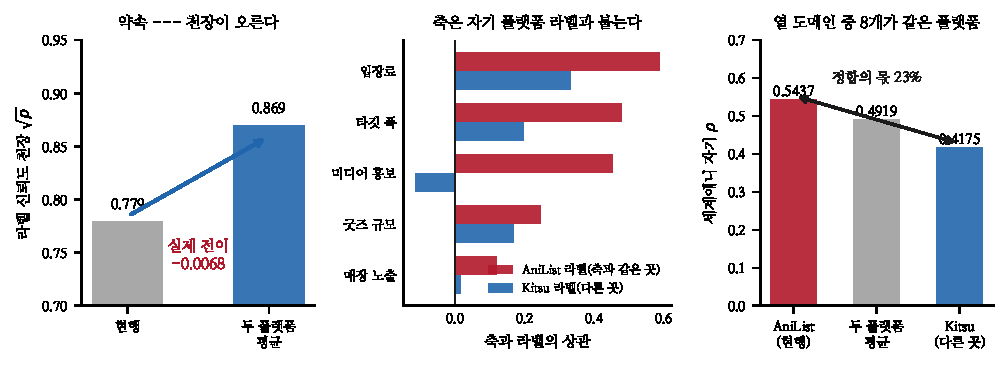
\includegraphics[width=\textwidth]{figs/ss.pdf}
\caption{왼쪽 --- 약속과 실제. 가운데 --- 축은 자기 플랫폼 라벨과 붙는다.
오른쪽 --- 정합의 몫.}
\end{figure*}

\section{천장이 오를 터였다}

\begin{table}[t]
\centering\tsize
\caption{두 플랫폼으로 라벨을 재면.}
\begin{tabular}{lr}
\toprule
AniList 라벨 vs Kitsu \texttt{userCount} & $+$0.607 \\
\quad(id 대응 2,892건) & \\
노트 79 · 83의 제목 대조 & $+$0.555 \\
\midrule
스피어만-브라운 $2\rho/(1{+}\rho)$ & 0.756 \\
천장 $\sqrt{\rho}$ & 0.779 $\to$ \textbf{0.869} \\
\bottomrule
\end{tabular}
\end{table}

\section{그런데 전이가 내린다}

\begin{table}[t]
\centering\tsize
\caption{세계애니를 \emph{출처}로 쓸 때. 대상 라벨은 안 바뀌므로 비교 가능하다.}
\begin{tabular}{lrrr}
\toprule
대상 & 현행 & 보정 후 & $\Delta$ \\
\midrule
애니 & $+$0.260 & $+$0.262 & $+$0.002 \\
만화 & $+$0.535 & $+$0.534 & $-$0.001 \\
도서 & $+$0.222 & $+$0.215 & $-$0.007 \\
웹툰 & $+$0.427 & $+$0.418 & $-$0.009 \\
\textbf{팝업} & $+$0.417 & $+$0.406 & \textbf{$-$0.011} \\
\textbf{모바일} & $+$0.495 & $+$0.475 & \textbf{$-$0.020} \\
\midrule
\multicolumn{3}{l}{평균(아홉 대상)} & \textbf{$-$0.0068} \\
\multicolumn{3}{l}{앙상블 팝업} & $-$0.0011 \quad 보류 4/4 \\
\bottomrule
\end{tabular}
\end{table}

\claimx{신뢰도를 올렸는데 전이가 내린다. \textbf{스피어만-브라운이 약속한 것이
안 온다.}}{보정 라벨은 2\%(Kitsu 가 없는 것)에서 원 라벨을 그대로 둔다. 그
불균질이 원인일 수는 없다 --- 방향이 아홉 중 여덟에서 같다.}

\section{축이 전부 같은 곳에서 나왔다}

\begin{table}[t]
\centering\tsize
\caption{세계애니의 축이 어느 라벨과 붙나.}
\begin{tabular}{lrr}
\toprule
& AniList 라벨 & Kitsu 라벨 \\
& (축과 같은 곳) & (다른 곳) \\
\midrule
입장료 & $+$0.587 & $+$0.331 \\
타깃 폭 & $+$0.486 & $+$0.197 \\
\textbf{미디어 홍보} & \textbf{$+$0.460} & \textbf{$-$0.113} \\
굿즈 규모 & $+$0.248 & $+$0.167 \\
매장 노출 & $+$0.122 & $+$0.017 \\
\bottomrule
\end{tabular}
\end{table}

세계애니의 축은 태그 수 · 화수 · 연령 등급 · 외부 링크 수 · 예고편이다 ---
\textbf{전부 AniList API 의 필드}다. 라벨(AniList 서재 등록 수)도 같은 API 다.

\claimx{\textbf{축이 자기 플랫폼의 라벨과 붙는다.} 다섯 축 전부 AniList 라벨과
더 세게 붙고, 미디어 홍보는 $+$0.460에서 $-$0.113으로 \textbf{부호까지}
뒤집힌다. AniList 의 외부 링크 수가 AniList 사용자의 목록 담기를 설명하는 만큼
Kitsu 사용자의 목록 담기를 설명하지 않는다.}{Kitsu 대응이 98\%지만 나머지
2\%가 어떤 작품인지 안 봤다. 마이너한 작품이 빠졌다면 Kitsu 쪽 상관이 낮게
나올 수 있다.}

\begin{table}[t]
\centering\tsize
\caption{세계애니 자기 $\rho$. 축은 셋 다 AniList 에서 나온 같은 것.}
\begin{tabular}{lrr}
\toprule
라벨 & $n$ & 자기 $\rho$ \\
\midrule
AniList popularity(현행) & 2,853 & \textbf{0.5437} \\
두 플랫폼 평균 & 2,853 & 0.4919 \\
\textbf{Kitsu userCount} & 2,817 & \textbf{0.4175} \\
\midrule
\multicolumn{2}{l}{같은 플랫폼 정합의 몫} & \textbf{23\%} \\
\bottomrule
\end{tabular}
\end{table}

\claimx{\textbf{자기 $\rho$의 23\%가 같은 플랫폼 정합이다.} 축과 라벨이 같은
API 에서 나오면 그 API 의 내부 구조(무엇을 태그로 다는지 · 어떤 작품에 링크를
많이 다는지)가 양쪽에 공통으로 들어간다. \textbf{정보가 아니라 정합이다.}}
{세계애니 하나에서 쟀다. 도메인마다 정합의 몫이 다를 것이다.}

\section{누수와 정합은 같은 것의 두 얼굴이다}

\begin{table}[t]
\centering\tsize
\caption{열 도메인의 축과 라벨 출처.}
\begin{tabular}{lll}
\toprule
& 축 & 라벨 \\
\midrule
게임 · 도서 · 펀딩 & 같은 플랫폼 & 같은 플랫폼 \\
웹툰 · 애니 · 모바일 & 〃 & 〃 \\
만화 · 세계애니 & 〃 & 〃 \\
\midrule
아이돌 & 한터/위키 & 한터 초동 \quad(일부) \\
\textbf{팝업} & \textbf{사람이 매김} & \textbf{결과보고서} \\
\bottomrule
\end{tabular}
\end{table}

\begin{quote}\fontsize{9.5}{11.5}\selectfont
노트 117에서 AniList 즐겨찾기가 AniList 라벨을 잘 맞힌 것을 \textbf{누수}라
부르고 판정에서 뺐다. 여기서 AniList 축들이 AniList 라벨을 잘 맞히는 것은
\textbf{정합}이라 부르고 그대로 쓴다. \textbf{정도의 차이일 뿐 종류가 같다.}
즐겨찾기는 상관 $+$0.855였고 축들은 $+$0.12$\sim+$0.59다.
\end{quote}

\claimx{\textbf{팝업만 다르다.} 팝업의 축은 사람이 기획서를 읽고 매기고 라벨은
결과보고서의 방문자 수다 --- 다른 출처, 다른 방법. \textbf{팝업의 자기
$\rho$($+$0.45$\sim$0.47)가 다른 도메인($+$0.54)보다 낮아 보이는 것은 팝업이
나빠서가 아니라 팝업만 정직하게 재지기 때문일 수 있다.} 세계애니를 정직한
눈금(Kitsu 라벨)으로 바꾸면 0.4175로 팝업과 같은 자리다.}{세계애니 하나의
23\%를 여덟 도메인에 일반화했다. 도메인마다 재 봐야 한다 --- 그러려면
도메인마다 다른 플랫폼의 라벨이 필요하다.}

\section{한계}

\begin{itemize}[leftmargin=1.1em,itemsep=0.15em]
\item \textbf{채택할 것이 없다.} 라벨 보정은 보류 4/4이고 방향이 음수다.
\item 정합의 몫 23\%를 세계애니 하나에서 쟀다.
\item ``팝업만 정직하다''는 아직 가설이다. 팝업의 축과 라벨이 다른 출처인
      것은 사실이지만 그것이 자기 $\rho$ 차이를 다 설명하는지는 모른다.
\item Kitsu 대응 98\%의 빠진 2\%를 안 봤다.
\item 다른 도메인에 다른 플랫폼 라벨을 안 붙였다 --- 붙이면 여덟 도메인의
      정직한 자기 $\rho$를 다 잴 수 있다.
\end{itemize}

\section{다음}

\begin{enumerate}[leftmargin=1.3em,itemsep=0.15em]
\item \textbf{정직한 눈금으로 다시 잰다} --- 도메인마다 다른 플랫폼의 라벨을
      붙여 자기 $\rho$를 다시 낸다. 만화도 Kitsu 가 있고, 게임은 SteamSpy,
      도서는 교보/예스24, 모바일은 구글플레이가 있다. \textbf{여덟 도메인의
      부풀림을 다 재면 이 프로젝트의 모든 수치가 다시 매겨진다.}
\item \textbf{팝업이 실은 최상위일 수 있다} --- 정직한 눈금에서 팝업의
      $+$0.46이 어디쯤인지. 노트 91의 도구 순위표가 바뀔 수 있다.
\item \textbf{팝업 레코드} --- 열세 노트가 같은 곳을 가리킨다.
\item 텀블벅 API --- 펀딩만 미디어 홍보 0\%다.
\end{enumerate}

\vspace{0.6em}
\hrule height 0.3pt
\vspace{0.5em}
{\footnotesize
\textbf{참고문헌}\\[0.3em]
Spearman, C. (1910). Correlation calculated from faulty data.
\emph{British Journal of Psychology}, 3(3), 271--295.\\[0.15em]
Brown, W. (1910). Some experimental results in the correlation of mental
abilities. \emph{British Journal of Psychology}, 3(3), 296--322.\\[0.15em]
Lord, F. M., Novick, M. R. (1968). \emph{Statistical Theories of Mental Test
Scores}. Addison-Wesley.\\[0.15em]
Kaufman, S. et al. (2012). Leakage in data mining: formulation, detection, and
avoidance. \emph{ACM TKDD}, 6(4), 1--21.\\[0.15em]
Ben-David, S. et al. (2010). A theory of learning from different domains.
\emph{Machine Learning}, 79(1--2), 151--175.
}

\end{document}
